\chapter{Transformações Lineares}
\thispagestyle{empty}

\section{Introdução}
O objetivo deste tópico é estudar funções (também chamadas de aplicações ou transformações) entre espaços vetoriais.  Estamos interessados particularmente em funções que preservem as operações de soma de vetores e multiplicação por escalar. As funções que satisfazem tais propriedades  são chamadas de transformações lineares. Estudaremos aqui apenas transformações lineares entre espaços vetoriais reais. No entanto, todos os conceitos apresentados são extensíveis à espaços vetoriais complexos.

\section{Transformação Linear}


\textbf{Definição (Transformação Linear).} Sejam $U$  e $V$ espaços vetoriais sobre o conjunto dos números reais.  Uma transformação linear de $U$ em $V$, $$T: U \rightarrow V$$  é uma função que possui as seguintes propriedades:
\begin{enumerate}[label=(\roman*)]
\item $T(u+v)=T(u)+T(v)$, para todo $u$ e $v$ em $U$.
\item $T(\alpha u )= \alpha T(u)$, para todo $u \in U$ e todo $\alpha \in \mathbb{R}$.
\end{enumerate}

\vspace{0.7cm}
\noindent \textbf{Observações.}

\begin{enumerate}
\item  {As propriedades $(i)$ e $(ii)$ são equivalentes à  $$ T(u+\alpha v)= T(u)+ \alpha T(v)$$ para todo $u$ e $v$ em $U$ e para todo $\alpha \in \mathbb{R}$ .}

\item Se $T: U \rightarrow V$ é uma transformação linear, então $$T(0_u)=0_v.$$
\end{enumerate}

As duas observações anteriores facilitam o trabalho de verificar se uma dada aplicação $T: U \rightarrow V$ é uma transformação linear, o que pode ser feito da seguinte maneira:  Primeiro, calculamos $T(0_u)$.    Se $T(0_u) \neq 0_v$, então  $T$ não pode ser uma transformação linear.  Agora,  caso $T(0_u)=0_v$,  então verificamos se  $T$  satisfaz $ T(u+\alpha v)= T(u)+ \alpha T(v)$ para todo $u$ e $v$ em $U$ e para todo $\alpha \in \mathbb{R}$. Em caso afirmativo, concluímos que $T$ é uma transformação linear de $U$ em $V$.

\vspace{0.3cm}

\section{Exemplos de Transformações Lineares}
\begin{enumerate}
\item A aplicação $T: \mathbb{R}^2 \rightarrow \mathbb{R}$ definida por $T(x,y)=x+y$ é uma transformação linear. De fato, $T(0,0)=0+0=0$. Além disso, sejam $u=(x_1,y_1)$ e $v=(x_2,y_2)$ vetores quaisquer do $\mathbb{R}^2$ e $\alpha$ um  número real qualquer. Note que $$u+ \alpha v=(x_1+\alpha x_2, y_1+\alpha y_2). $$  Assim,  $$T(u+\alpha v)=T(x_1+\alpha x_2, y_1+\alpha y_2)=(x_1+\alpha x_2)+ (y_1+\alpha y_2)=(x_1+y_1)+\alpha ( x_2+y_2).$$ Por outro lado, como $T(u)= x_1+y_1$ e $T(v)=x_2+y_2$, então  $$T(u)+ \alpha T(v)= x_1+y_1+ \alpha(x_2+y_2).$$ Portanto,
$ T(u+\alpha v)= T(u)+ \alpha T(v)$.

\item A aplicação $T: \mathbb{R}^2 \rightarrow \mathbb{R}^2$ definida por $T(x,y)=(x+y, x+1)$ não  é uma transformação linear. De fato, $T(0,0)=(0,1) \neq (0,0)$.

\item A aplicação $T: \mathbb{R}^2 \rightarrow \mathbb{R}^3$ definida por $T(x,y)=(x,x+y,y)$ é uma transformação linear. De fato, $T(0,0)=(0,0,0)$. Além disso, sejam $u=(x_1,y_1)$ e $v=(x_2,y_2)$ vetores quaisquer do $\mathbb{R}^2$ e $\alpha$ um  número real qualquer.  $$T(u+\alpha v)=T(x_1+\alpha x_2, y_1+\alpha y_2)=(x_1+\alpha x_2, x_1+\alpha x_2+ y_1+\alpha y_2,  y_1+\alpha y_2). $$ Por outro lado,   como $T(u)=(x_1,x_1+y_1,y_1$ e $T(v)=(x_1, x_2+y_2, y_2)$, então    $$T(u)+\alpha T(v)=(x_1, x_1+y_1, y_1)+\alpha ( x_2,  x_2+y_2, y_2)=(x_1+\alpha  x_2, x_1+y_1+ \alpha ( x_2+ y_2), y_1 + \alpha y_2).$$   Portanto, $T(u+\alpha v)=T(u)+\alpha T(v).$

\item A aplicação $T: \mathbb{R}^3 \rightarrow \mathbb{R}^3$ definida por $T(x,y, z)=(x,y,z)$ é uma transformação linear. De fato, $T(0,0, 0)=(0,0,0)$. Além disso, sejam $u=(x_1,y_1, z_1)$ e $v=(x_2,y_2, z_2)$ vetores quaisquer do $\mathbb{R}^3$ e $\alpha$ um  número real qualquer.  Note que $$u+ \alpha v=(x_1+\alpha x_2, y_1+\alpha y_2, z_1+\alpha z_2). $$
Dessa  maneira,
 $$T(u+\alpha v)=T(x_1+\alpha x_2, y_1+\alpha y_2, z_1+\alpha z_2)=(x_1+\alpha x_2, y_1+\alpha y_2, z_1+\alpha z_2). $$ Por outro lado, $$T(u)+\alpha T(v)=(x_1, x_1, z_1)+\alpha ( x_2,  x_2, z_2)=(x_1+\alpha x_2, y_1+\alpha y_2, z_1+\alpha z_2).$$ Portanto, $ T(u+\alpha v)=T(u)+\alpha T(v)$.

\item  A aplicação $T: \mathbb{R}^3 \rightarrow \mathbb{M}(2, 2)$ definida por $$T(x,y, z)= \left[ \begin{array}{cc} x & 3\\ x-y & z-x \end{array} \right]$$  não  é uma transformação linear. De fato, $T(0,0, 0)= \left[ \begin{array}{cc} 0 & 3\\ 0 & 0 \end{array} \right] \neq \left[ \begin{array}{cc} 0 & 0\\ 0 & 0 \end{array} \right]$.

\item  A aplicação $T: \mathbb{R}^2 \rightarrow \mathbb{R}^2$ definida por $$T(x,y)=(xcos\theta - ysen\theta,xsen\theta+ ycos\theta)$$
% \left[ \begin{array}{cc} xcos\theta & ysen\theta \\ -xsen\theta & ycos\theta \end{array} \right]$$
é uma transformação linear. Com efeito, dados  $u=(x_1,y_1)$ e $v=(x_2,y_2)$ vetores quaisquer do $\mathbb{R}^2$ e $\alpha \in \mathbb{R}$, temos:

\begin{align*}
T(u+\alpha v) &= T(x_1+\alpha x_2, y_1+\alpha y_2) \\
                        &= ((x_1+\alpha x_2)cos\theta - (y_1+\alpha y_2)sen\theta, (x_1+\alpha x_2)sen\theta+ (y_1+\alpha y_2)cos\theta)\\
                       &=  (x_1cos\theta - y_1sen\theta, x_1sen\theta+ y_1cos\theta)+(\alpha x_2cos\theta - \alpha y_2sen\theta, \alpha x_2sen\theta+ \alpha y_2cos\theta)\\
                      &=  (x_1cos\theta - y_1sen\theta, x_1sen\theta+ y_1cos\theta)+\alpha( x_2cos\theta -  y_2sen\theta,  x_2sen\theta+ y_2cos\theta))\\
                       &=T(u)+\alpha T(v).
%\left[ \begin{array}{cc} (x_1+\alpha x_2)cos\theta & (y_1+\alpha y_2) sen\theta \\ -(x_1+\alpha x_2)sen\theta & (y_1+\alpha y_2)cos\theta \end{array} \right] \\
%&=  ((x_1+\alpha x_2)cos\theta - (y_1+\alpha y_2)sen\theta, (x_1+\alpha x_2)sen\theta+ (y_1+\alpha y_2)cos\theta)\\ %\left[ \begin{array}{cc} x_1cos\theta & y_1 sen\theta \\ -x_1sen\theta & y_1cos\theta \end{array} \right] + \alpha \left[ \begin{array}{cc}  x_2cos\theta & y_2 sen\theta \\ -x_2sen\theta & y_2cos\theta \end{array} \right]\\
%&=T(u)+\alpha T(v).
\end{align*}


\item A aplicação $T: \mathcal{P}_2(\mathbb{R}) \rightarrow \mathbb{R}^3$ definida por $$T(a_0+a_1x+a_2x^2)=(a_0, a_1, a_2)$$ é uma transformação linear. Com efeito, sejam $p(x)=a_0+a_1x+a_2x^2$ e $q(x)=b_0+b_1x+b_2x^2$ polinômios quaisquer do espaço vetorial $\mathbb{P}_2(\mathbb{R})$ e $\alpha \in \mathbb{R}$.  Da soma de dois polinômios obtemos $$p+\alpha q=a_0+\alpha b_0+(a_1+\alpha b_1)x+(a_2+\alpha b_2)x^2.$$ Assim, $$T(p+\alpha q)=T(a_0+\alpha b_0+(a_1+\alpha b_1)x+(a_2+\alpha b_2)x^2)=(a_0+\alpha b_0, a_1+\alpha b_1, a_2+\alpha b_2).$$
Por outro lado, como $T(p)=(a_0, a_1,a_2)$ e $T(q)=(b_0, b_1, b_2))$, então  $$T(p) +\alpha T(q)=(a_0, a_1, a_2) + \alpha ( b_0, b_1, b_2)=(a_0+\alpha b_0, a_1+\alpha b_1, a_2+\alpha b_2).$$ Logo, $ T(p+\alpha q)=T(p)+\alpha T(q)$.

\item Seja $D: \mathcal{P}_3(\mathbb{R}) \rightarrow \mathcal{P}_2(\mathbb{R})$ uma transformação do espaço dos polinômios de grau menor ou igual a 3 no espaço dos polinômios de grau menor ou igual a 2, ambos sobre $\mathbb{R}$, tal que $$D(a_3x^3+a_2x^2+a_1x+a_0)=3a_3x^2+2a_2x+a_1.$$ Isto é, $\mathcal{D}$ é a função derivada restrita ao espaço vetorial $\mathcal{P}_3(\mathbb{R})$. Como a derivada da soma de duas funções é a soma das derivadas dessas funções; e a derivada do produto de uma constante por uma função é igual a constante vezes a derivada da função, então podemos afirmar que $D$ é uma transformação linear de $\mathcal{P}_3(\mathbb{R})$ em $ \mathcal{P}_2(\mathbb{R})$.

\item Seja $\mathcal{C}([a,b], \mathbb{R})$ o conjunto formado por todas as funções reais  $f: [a,b] \rightarrow \mathbb{R}$ contínuas em $[a,b]$. A transformação  $S: \mathcal{C}([a,b], \mathbb{R}) \rightarrow \mathbb{R}$ tal que $$S(f)=\int_{a}^{b}f(x)dx$$ é uma transformação linear. De fato, a constatação deste fato é uma consequências das propriedades das integrais definidas.
\end{enumerate}

%\section{Exercícios Propostos}
\section{Exercícios Propostos}
\begin{enumerate}
\item Seja $V$ um espaço vetorial real qualquer. Mostre que $T: V \rightarrow V$   dada por $T(v)=v$ é uma transformação linear.

\item Seja $T: \mathbb{R} \rightarrow  \mathbb{R}$ uma aplicação definida por $T(x)=\lambda x$. Mostre que $T$ é linear. (Na verdade,  toda transformação linear de  $\mathbb{R}$ em $ \mathbb{R}$ é da forma $\lambda x$. Mostre isso!).
\item Mostre que as seguintes aplicações de $\mathbb{R}^2$ em $\mathbb{R}^2$ são transformações lineares.

\begin{enumerate}[label=(\alph*)]
\item  $T: \mathbb{R}^2 \rightarrow \mathbb{R}^2$ definida por $T(x,y)=c(x,y)$ para todo $c \in \mathbb{R}$ (\textit{Contração ou expansão}).
\item  $T: \mathbb{R}^2 \rightarrow \mathbb{R}^2$ definida por $T(x,y)=(x,-y)$  (\textit{Reflexão em torno do eixo x}).
\item  $T: \mathbb{R}^2 \rightarrow \mathbb{R}^2$ definida por $T(x,y)=(-x,-y)$  (\textit{Reflexão na origem}).
\item  $T: \mathbb{R}^2 \rightarrow \mathbb{R}^2$ definida por $T(x,y)=(x+cy,y)$ para todo $c \in \mathbb{R}$ (\textit{Cisalhamento horizontal}).
\end{enumerate}

\item Sejam $a$ e $b$ números reais diferentes de zero.  Mostre que  $T: \mathbb{R}^2 \rightarrow \mathbb{R}^2$ definida por $T(x,y)=(x+a,y+b)$ (\textit{Translação}) não é uma transformação linear.

\item  Mostre que a aplicação $T: \mathbb{R}^2 \rightarrow \mathbb{M}(2, 2)$ definida por $$T(x,y)= \left[ \begin{array}{cc} x+y & x\\ y & x-y \end{array} \right]$$   é uma transformação linear.



\item Seja $P \in \mathbb{M}(2, 2)$ uma matriz invertível e $T_P: \mathbb{M}(2, 2) \rightarrow \mathbb{M}(2, 2)$, definida por $$T_P(X)=P^{-1}XP.$$ Mostre que $T_P$ é linear.

\item Sejam $U$ e $V$ espaços vetoriais  quaisquer.  Se  $T: U \rightarrow V$   é uma transformação linear, mostre que $T(0_u)=0_v$.

\item {Sejam $V$ e $W$ espaços vetoriais  sobre $\mathbb{R}$ e $T : V \rightarrow W$ uma transformação linear. Mostre que se  $\{T(v_1),T( v_2),...,T(v_n)\}$ é um conjunto linearmente independente de $W$, então $\{v_1, v_2,...,v_n\}$ é um conjunto linearmente independente de $V$.}

\end{enumerate}

\section{Determinando uma transformação linear a partir da imagem dos vetores de uma base do domínio}
 Uma característica muito importante das transformações lineares é que uma transformação linear fica univocamente determinada se conhecemos seus valores nos vetores de uma base do domínio. Esse resultado é consequência do seguinte teorema:

\vspace{0.3cm}
\noindent \textbf{Teorema 1.} \textit{Sejam $\{ u_1, u_2, ..., u_n\}$ uma base de um espaço vetorial  $U$. Sejam $\{ v_1, v_2,..., v_n\}$ vetores de um espaço vetorial $V$. Então, existe uma única transformação linear  $T: U \rightarrow V$ tal que $T(u_i)=v_i$ para $i=1,2, ..., n$. }

\vspace{0.3cm}
\noindent \textbf{Observação.} Esta aplicação é dada por: se $$ u=a_1u_1+a_2u_2+...+a_nu_n,$$  então  $$T(u)=a_1T(u_1)+a_2T(u_2)+...+a_nT(u_n)=a_1v_1+a_2v_2+...+a_nv_n.$$

Além de afirmar a existência de uma única transformação linear satisfazendo certas condições, o teorema anterior, e a observação anterior, nos fornecem um roteiro de como determinar uma transformação linear $T: U \rightarrow V$ conhecendo-se uma base de $U$,  $\{ u_1, u_2, ..., u_n\}$, e  $n$ vetores de $V$, $\{ v_1, v_2,..., v_n\}$ , tais que $T(u_i)=v_i$ para $i=1,2, ..., n$.
\begin{enumerate}
\item Certifique-que $u_1, u_2,...,u_n$ formam uma base de $U$;
\item Escreva um vetor genérico de  $u \in U$ como uma combinação linear de $u_1, u_2,...,u_n$. Isto é, calcule escalares $a_1, a_2,...,a_n$ tais que $$u=a_1u_1+ a_2u_2+...+a_nu_n;$$
\item Escreva a equação $T(u)=a_1T(u_1)+ a_2T(u_2)+...+a_nT(u_n)$;
\item Faça a substituição $T(u_i)=v_1$ para $i=1,2,...,n$.
\item Organize os cálculos e escreva a expressão para $T(u)$,  onde $u$ é um vetor qualquer de $U$.
\end{enumerate}

\section{ Exemplo}
Dada uma base qualquer de $\mathbb{R}^2$, por exemplo, $\beta=\{(1,1), (-1, 1)\}$,  e dois vetores quaisquer de  $\mathbb{R}^3$, por exemplo, $( 1, -1,1)$ e $(0, 1,2)$.  O teorema anterior afirma que existe uma única transformação linear $T: \mathbb{R}^2 \rightarrow \mathbb{R}^3$ tal que $$T(1,1) = (1, -1, 1)$$ e  $$T(-1, 1) =(0, 1, 2).$$
Além disso, como dado $(x,y) \in \mathbb{R}^2$, sempre vai existir escalares $a_1$ e $a_2$ únicos, tais que,  $(x,y)= a_1(1, 1)+ b_1(-1, 1)$, então  a  transformação linear $T$ é dada por $$T(x,y)= a_1T(1, 1)+ b_1T(-1, 1)= a_1(1,-1,1)+a_2(0, 1,2).$$
Dessa maneira, para encontrarmos uma fórmula para $T$ basta apenas calcularmos os escalares $a_1$ e $a_2$. Isso pode ser feito, resolvendo-se o sistema $$(x,y)= a_1(1, 1)+ b_1(-1, 1).$$
Ou seja,
\begin{align*}
x &=a_1-b_1 \\
y&=a1+b1.
\end{align*}

Daí  obtemos $a_1=\dfrac{x+y}{2}$ e $a_2=\dfrac{y-x}{2}$. Dessa maneira,
\begin{align*}
T(x,y)&= \dfrac{x+y}{2}(1,-1,1)+\dfrac{y-x}{2}(0, 1,2)\\
          &=\left(\dfrac{x+y}{2}, -x, \dfrac{-x+3y}{2}\right).
\end{align*}

Portanto, a transformação linear procurada é



 $$T(x,y)= \left(\dfrac{x+y}{2}, -x, \dfrac{-x+3y}{2}\right).$$

\section{Exercícios Propostos}
\begin{enumerate}

\item Seja $T: \mathbb{R}^2 \rightarrow \mathbb{R}^2$  uma transformação linear tal que $T(1,0)=(1,1)$ e $T(0,1)=(-1,1)$.
\begin{enumerate}[label=(\alph*)]
\item Determine $T(x,y)$.
\item Calcule $T(2,3)$.
%\item Descreva $Ker(T)$ e $Im(T)$.
\end{enumerate}

\item Seja $T: \mathbb{R}^3 \rightarrow \mathbb{R}^3$  uma transformação linear tal que $T(1,0,0)=(2,-1,1)$,  $T(1,1, 0)=(-1,2,1)$  e $T(1,1, 1)=(1,1,-2)$ .
\begin{enumerate}[label=(\alph*)]
\item Determine $T(x,y,z)$.
\item Calcule $T(2,3,1)$.
%\item Descreva $Ker(T)$ e $Im(T)$.
\end{enumerate}

\item Seja  Seja $T: \mathbb{R}^3 \rightarrow \mathbb{R}$ tal que  $T(1,-1,1)=1$,  $T(1,0, 2)=2 $  e $T(1,1, 1)=3$ . Determine $T(x,y,z)$.
%\begin{enumerate}[label=(\alph*)]
%\item  $T(x,y)$.
%\item $Ker(T)$.
%\end{enumerate}

\item Seja $T: \mathbb{R}^4 \rightarrow \mathbb{R}^2$  uma transformação linear tal que  $T(1,0,0, 0)=(1,1)$, $T(1,1,0,0)=(-1,1)$,  $T(0,1,1, 0)=(1,-1)$ e   $T(0,0,1, 1)=(-1,-1)$ .
\begin{enumerate}[label=(\alph*)]
\item Determine $T(x,y,z,t)$.
\item Calcule $T(1,2,2,3)$.
%\item Descreva $Ker(T)$ e $Im(T)$.
\end{enumerate}

\item Seja $T: \mathbb{P}_2(\mathbb{R}) \rightarrow \mathbb{R}^3$  uma transformação linear tal que  $T(1+2x+x^2)=(1,2,1)$, $T(1+x)=(1,-1,-2)$ e  $T(2)=(1,0,0)$. Determine $T(a_0+a_1x+a_2x^2)$.
\end{enumerate}

\section{Núcleo e Imagem}
\textbf{Definição (Núcleo e Imagem).} \textit{Sejam $U$  e $V$ espaços vetoriais e $T: U \rightarrow V$ uma transformação linear. }

\begin{enumerate}%[label=(\roman*)]
\item \textit{O conjunto $\{ u\in U; \;T(u)=0_v\}$ é chamado de \textit{Núcleo de $T$} e será denotado por \textit{Ker(T)}.}

\begin{figure}[h]
\center
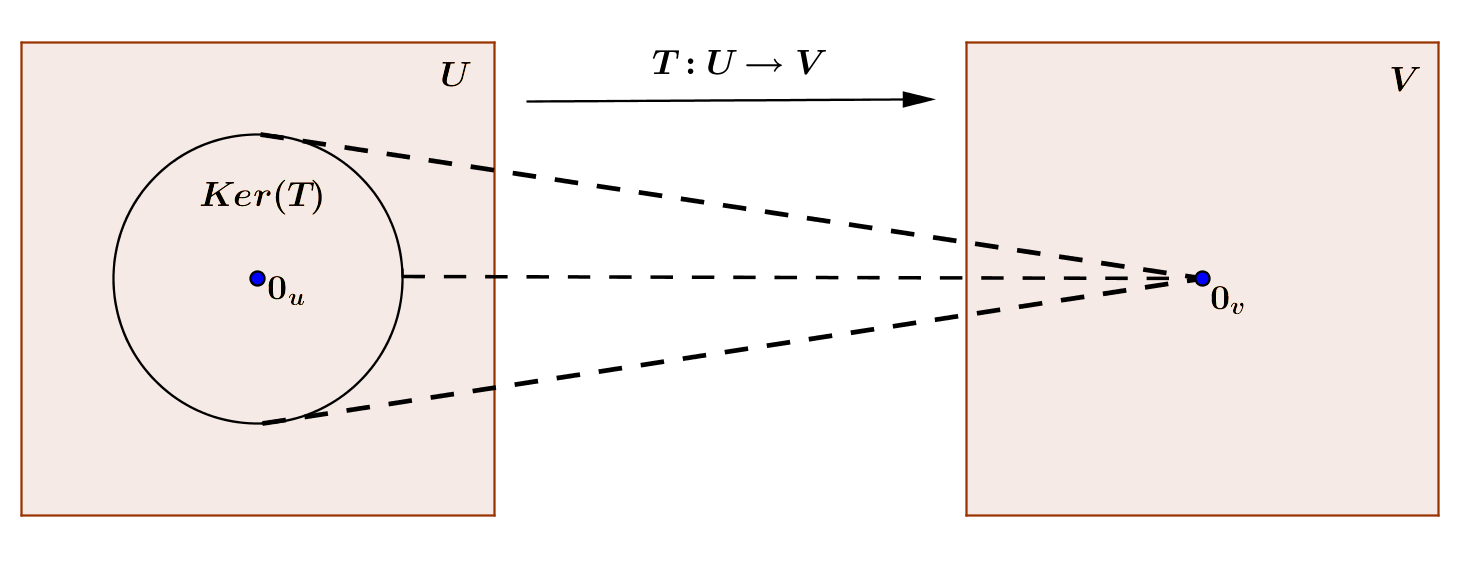
\includegraphics[width=0.70\textwidth]{chapters/transformacoes_lineares/img/kert1}
\caption{\footnotesize{Cada vetor $u \in Ker(T)$ é levado  em $0_v$ por  T .}}
\label{fig:exp}
\end{figure}


\item \textit{O conjunto $\{ v \in V;  \; v=T(u) \; \; \text{para algum}\; u\in U\}$ é chamado de \textit{Imagem de $T$} e será denotado por \textit{Im(T)}, ou simplesmente $T(U)$.}

\begin{figure}[h!]
\center
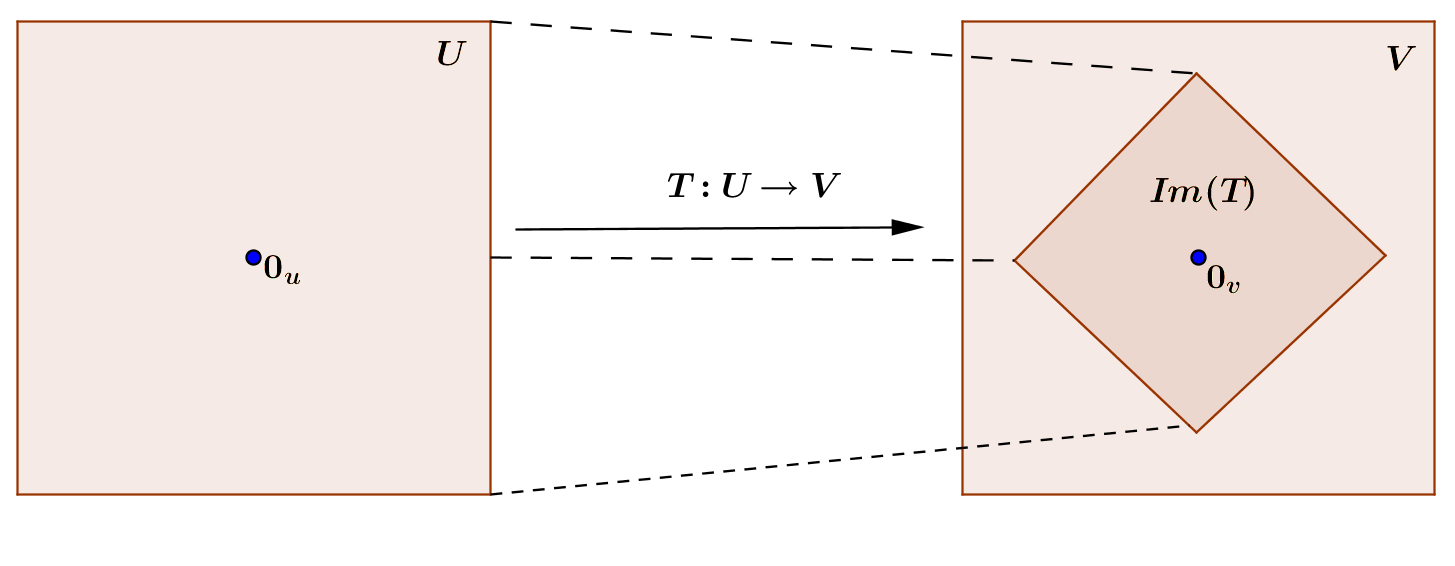
\includegraphics[width=0.70\textwidth]{chapters/transformacoes_lineares/img/imt1}
\caption{\footnotesize{Representação gráfica da imagem de T.}}
\label{fig:exp}
\end{figure}

\end{enumerate}

Observe que tanto \textit{Ker(T)} como \textit{Im(T)} são conjuntos diferentes do vazio. Isto porque, como já  sabemos,  $T(0_u)=0_v$. Logo, cada um desses conjuntos têm pelo menos o elemento nulo. Dessa forma, é conveniente investigar se esses conjuntos possuem a estrutura de um espaço vetorial. A resposta a essa pergunta é dada pelo \textbf{Teorema 2}.





\vspace{1cm}
\noindent \textbf{Teorema 2.} \textit{Seja $T: U \rightarrow V$ uma transformação linear. Então, \textit{Ker(T)} é um subespaço vetorial de $U$ e \textit{Im(T)} é um subespaço vetorial de $V$.}

\noindent \textbf{Demonstração.} Primeiro vamos mostrar que \textit{Ker(T)} é um subespaço vetorial de $U$. Para isso, sejam $u_1$ e $u_2$ dois vetores quaisquer de  \textit{Ker(T)} e $\lambda \in \mathbb{R}$. Vamos mostrar que $u_1+\lambda u_2 \in{Ker(T)} $. De fato, $$T(u_1+\lambda u_2)=T(u_1)+\lambda T(u_2)$$ pois $T$ é linear. Mas, como $u_1$ e $u_2$ pertencem  a  \textit{Ker(T)},  temos $T(u_1)=0_v$ e $T(u_2)=0_v$. Daí, $$T(u_1+\lambda u_2)=0_v+\lambda 0_v=0_v.$$ Logo,   $u_1+\lambda u_2 \in{Ker(T)} $ e, portanto, \textit{Ker(T)} é um subespaço vetorial de $U$.

Agora para mostrar que \textit{Im(T)} é um subespaço vetorial de $V$, considere dois vetores genéricos  $v_1$ e $v_2$ em \textit{Im(T)}. Daí, pela definição da \textit{Im(T)}, existem vetores $u_1$ e $u_2$ no domínio da transformação tais que
$$v_1=T(u_1) \; \text{e} \; v_2=T(u_2).$$

Assim, para todo $\lambda \in \mathbb{R}$, temos $$v_1+\lambda v_2=T(u_1) +\lambda T(u_2).$$ Como $T$ é linear, então
$$v_1+\lambda v_2=T(u_1 +\lambda u_2).$$ Isso mostra que $v_1+\lambda v_2 \in Im(T)$, pois é imagem do vetor $u_1 +\lambda u_2 \in U$. Portanto, $Im(T)$ é um subespaço vetorial de $V$.

\vspace{1cm}

A seguir veremos como calcular o núcleo e a imagem de uma transformação linear por meio de alguns exemplos.

\section{Exemplos}
\begin{enumerate}
\item Considere a transformação linear $T: \mathbb{R}^2 \rightarrow \mathbb{R}^4$ definida por $$T(x,y)=(x, y,x+y, x-y).$$  Para determinar  $Ker(T)$  note que  $(x,y) \in Ker(T)$ se, e somente se, $T(x,y)=(0,0)$. Mas isso implica em $(x, y, x+y, x-y)=(0,0,0,0)$. Logo, devemos ter $x=0$, $y=0$, $x+y=0$ e $x-y=0$. Obviamente, $x=y=0$. Assim obtemos,  $$Ker(T)=\{(0,0)\}.$$ Agora, para calcular $Im(T)$, note que cada elemento de $\mathbb{R}^4$ que está na imagem de $T$ é dado pela transformação $T(x,y)=(x, y, x+y, x-y)$.  Assim, fazemos $$(x,y,x+y, x-y)=x(1,0,1,1)+y(0,1,1,-1).$$ Dessa maneira, $$Im(T)=[(1,0,1,1),(0,1,1,-1)].$$

\item Considere a  transformação linear $T: \mathbb{R}^3 \rightarrow \mathbb{R}^2$ definida por $T(x,y,z)=(x, y)$. O vetor $(x,y,z) \in Ker(T)$ se, e somente se, $T(x,y,z)=(0,0)$. Mas isso implica em $(x, y)=(0,0)$. Logo, devemos ter $x=0$ e $y=0$. Mas, não encontramos nenhuma restrição sobre a variável  $z$. Ou seja, $z$ é  livre. Assim obtemos,  $$Ker(T)=\{(0,0, z); \; z \in \mathbb{R}\}.$$

Já $Im(T)$ pode ser obtida através de $$T(x, y)=(x,z)=x(1,0)+y(0,1).$$ Logo, $$Im(T)=[(1,0), (0,1)]=\mathbb{R}^2.$$
\end{enumerate}

\section{Exercícios Propostos}
\begin{enumerate}
\item  Para cada uma das transformações lineares dos exercícios da \textbf{Seção 6}
\begin{enumerate}[label=(\alph*)]
\item Calcular $Ker(T)$.
\item Descrever $Im(T)$.
\end{enumerate}
\item Determine o núcleo e a imagem da transformação linear $T: \mathbb{R}^4 \rightarrow \mathbb{R}^2$ definida  por $T(x,y,z,w)=(x-y, y-z, z-w)$.

\item Demonstre o Teorema 2.
\end{enumerate}

\section{Transformações Lineares Injetivas e Sobrejetivas}

Uma função  $T: U \rightarrow V$ é \textit{injetiva} (ou injetora)  se  $$T(x)=T(y) \Rightarrow x=y,\; \text{para todo}\; x, y \in U.$$ Isto equivale a dizer que numa função injetiva  as imagens de elementos distintos são distintas.

 Por outro lado, $T$ é uma função \textit{sobrejetiva} (ou sobrejetora) se $Im(T)=V$. Isto é, todo elemento do contradomínio $V$ é  imagem de algum elemento do domínio $U$. Se uma função $T$ é injetiva e sobrejetiva,  dizemos que $T$ é \textit{bijetiva} (ou bijetora).

Por exemplo, a função $f: \mathbb{R} \rightarrow \mathbb{R}$ dada por $f(x)=x^2$ não é injetora, pois $f(-2)=f(2)=4$. Ou seja, dois elementos distintos do domínio, -2 e 2,  possuem a mesma imagem 4.  Esta função também não  é sobrejetiva, pois $f(x)=x^2 \geq 0$ para todo $x\in \mathbb{R}$. Logo, $Im(f)=[0, \infty) \neq \mathbb{R}$. Já a função $f: \mathbb{R} \rightarrow \mathbb{R}$ dada por $f(x)=x^3$ é injetiva e sobrejetiva. Com efeito, $$f(x)=f(y) \Rightarrow x^3=y^3 \Rightarrow x^3 - y^3=0 \Rightarrow (x-y)(x^2+xy+y^2)=0$$ como $x^2+xy+y^2 > 0$ sempre que $x^2+y^2 \neq 0$, então $x-y=0$. Logo, $x=y$ e portanto $f$ é injetora. É simples verificar que $Im(f)=\mathbb{R}$, logo $f$  é sobrejetiva.

\vspace{1cm}
A tarefa de identificar se uma função $T$ é injetiva, em  geral, é  mais simples se $T$ é uma transformação linear.  Isso porque, conforme o \textbf{Teorema 3} que será apresentado a seguir, o trabalho de identificar se $T$ é injetiva fica reduzido a calcular o $Ker(T)$.  Esta  importante relação entre o núcleo de uma transformação linear e o fato da mesma  ser ou não  injetiva é estabelecida pelo seguinte teorema:

\vspace{1cm}
\noindent \textbf{Teorema 3.} \textit{Seja $T: U \rightarrow V$ uma transformação linear. Então, $T$ é uma aplicação injetiva se, e somente se, $Ker(T)=\{0_u\}.$}

\vspace{0.3cm}
\noindent \textbf{Demonstração.} Primeiro, suponha que $T$ é uma transformação linear injetiva e seja $u\in Ker(T)$. Então, por definição $T(u)=0_v$. Mas, já sabemos que  $T(0_u)=0_v$. Assim, $T(u)=T(0_u)$. Como $T$ é injetiva, $u=0_u$. Como o vetor $u$ foi tomado de modo arbitrário, segue que o único vetor no $ Ker(T)$ é o vetor nulo $0_u$. Ou seja, $ Ker(T)= \{0_u\}$.

Por outro lado, suponha que  $ Ker(T)= \{0_u\}$ e sejam vetores quaisquer $u_1$ e $u_2$ em $U$, tais que $T(u_1)=T(u_2)$. Vamos mostrar que $u_1=u_2$. De fato, se $T(u_1)=T(u_2)$, temos $T(u_1)-T(u_2)=0_v$. Mas, como $T$ é linear, segue que $T(u_1-u_2)=0_v$. Logo, $u_1-u_2 \in Ker(T)$. Mas, como $ Ker(T)= \{0_u\}$, então $u_1-u_2=0_u$. Logo, $u_1=u_2$. Portanto, de acordo com a definição de função injetiva,  $T$ é injetiva.




\vspace{1cm}

\section{Exemplos}


\begin{enumerate}
\item  A transformação linear $T: \mathbb{R}^2 \rightarrow \mathbb{R}^2$ definida por $T(x,y)=(x+2y,y)$ é injetiva. Com efeito, de acordo com a definição de núcleo $(x,y) \in Ker(T)$ se, e somente se, $T(x,y)=(0,0)$. Mas isso implica em $(x+2y, y)=(0,0)$. Logo, $x+2y=0$ e $y=0$ e assim obtemos, $x=y=0$. Portanto,  $Ker(T)=\{(0,0)\}$ e $T$ é injetiva, segundo o teorema.

\item A transformação linear $T: \mathbb{R}^3 \rightarrow \mathbb{R}$ definida por $T(x,y,z)=x+y+z$ não é injetiva. De fato, de acordo com a definição de núcleo $(x,y,z) \in Ker(T)$ se, e somente se, $T(x,y,z)=0$. Mas isso implica em $x+y+z=0$. De onde obtemos  $z=-x-y$. Assim, as variáveis $x$ e $y$ são livres e podem assumir qualquer valor real. Dessa forma   $$Ker(T)=\{(x,y, -x-y); x, y \in \mathbb{R}\} \neq \{ (0,0,0)\}.$$  Logo,  $T$ não é injetiva.

\end{enumerate}

\section{Exercícios Propostos}

\begin{enumerate}

\item Considere a transformação linear  $T: \mathbb{R}^3 \rightarrow \mathbb{R}^3$ definida por $T(x,y,z)=(x,x, z-y)$.

\begin{enumerate}[label=(\alph*)]
\item Determine $Ker(T)$. $T$ é injetiva?
\item Determine uma base para $Ker(T)$.
\item Determine uma base para $Im(T)$. Qual a dimensão de $Im(T)$.
\item $T$ é sobrejetiva?
\end{enumerate}

\item Sejam $U$ e $V$ espaços vetoriais e  $\{u_1, u_2,...,u_n\}$  um conjunto de vetores linearmente independentes de $U$. Mostre que, se $T: U \rightarrow V$ é uma transformação linear injetiva, então  $\{T(u_1), T(u_2),...,T(u_n)\}$  é um conjunto de vetores linearmente de $V$ (Isto é, transformações lineares injetivas levam conjunto LI em conjunto LI).
\end{enumerate}

\section{O Teorema do Núcleo e da Imagem. Isomorfismos}

O próximo teorema é um dos mais importantes da Álgebra Linear. Ele relaciona as dimensões do núcleo e da imagem de uma transformação linear  $T: U \rightarrow V$  com  a dimensão do espaço $U$ (o domínio da transformação linear). Esse teorema traz consequências interessantes para a análise de transformações injetivas e sobrejetivas, como veremos nas próximas seções.

\vspace{1cm}
\noindent \textbf{Teorema 4 (Teorema do Núcleo e da Imagem).} \textit{Sejam $U$ e $V$ espaços vetoriais, sendo $U$ de dimensão finita,  e  $T: U \rightarrow V$ uma transformação linear. Então, $$dim(Ker(T)) + dim(Im(T))=dim(U).$$}

\noindent\textit{Demonstração. Aula}


Para avaliarmos um pouco a importância do \textbf{Teorema 4},  considere uma transformação  linear $T: \mathbb{R}^3 \rightarrow \mathbb{R}^2$. O Teorema do Núcleo e da Imagem afirma que $$dim( \mathbb{R}^3 ) =3=dim(Ker(T))+ dim(Im(T)).$$ Isto é, a soma da dimensão do núcleo de $T$ com a dimensão da imagem de $T$ tem que ser exatamente 3. Mas, como $Im(T) \subset \mathbb{R}^2$, a dimensão da imagem de $T$ é no máximo igual a 2. Logo, a dimensão do núcleo de $T$ deve ser maior ou igual a 1. Portanto, $Ker(T)\neq \{ 0_u\}$. Dessa maneira, concluimos que  $T$ não pode ser injetora. Esse raciocínio se aplica a todas as transformações lineares  $T: U \rightarrow V$  tais que $dim(U) > dim(V)$. No caso em que $dim(U) = dim(V)$, temos o seguinte resultado:


\vspace{1cm}
\noindent\textbf{Corolário 1.} \textit{Sejam $U$  e $V$ espaços vetoriais de dimensão finita e    $T: U \rightarrow V$ uma transformação linear. Se $dim(U)=dim(V)$, então  $T$ é injetiva se, e somente se, $T$ é sobrejetiva.}

\vspace{1cm}
\noindent\textbf{Definição (Isormorfismo).} Sejam $U$  e $V$ espaços vetoriais.
\begin{enumerate}%[label=(\roman*)]
\item Se $T: U \rightarrow V$  é uma transformação linear bijetiva, $T$ é chamada de \textit{isomorfismo}.
\item Quando existe um isomorfismo  $T: U \rightarrow V$, dizemos que $U$ e $V$ são espaços vetoriais \textit{isomorfos} e denotamos $U \simeq V$.
\end{enumerate}

\begin{figure}[h]
\center
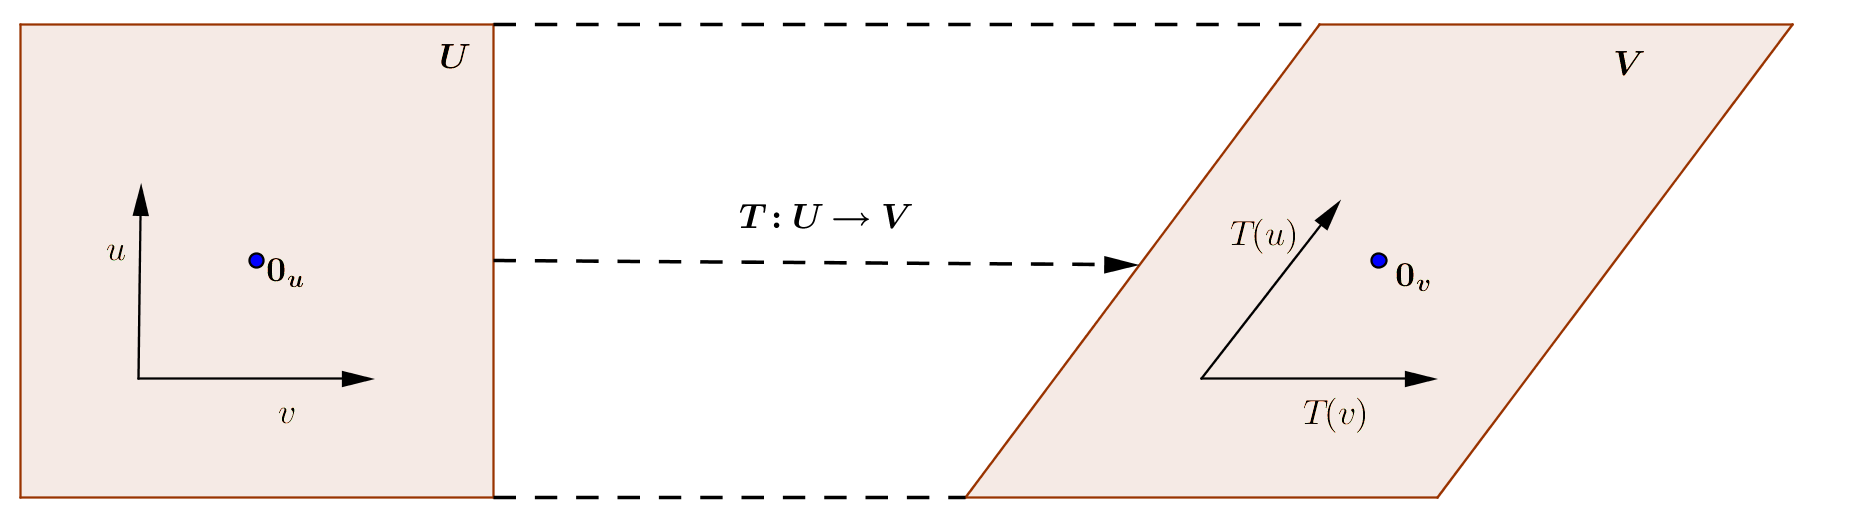
\includegraphics[width=0.70\textwidth]{chapters/transformacoes_lineares/img/isomorfismo}
\caption{\footnotesize{Espaços isomorfos possuem a mesma estrutura vetorial }}
\label{fig:exp}
\end{figure}

Espaços vetoriais isomorfos são essencialmente  iguais. A diferença está apenas na forma de representação dos seus vetores e das operações de soma de vetores e mutiplicação de vetores por escalar. Espaços vetoriais isomorfos devem ter a mesma dimensão.  Outras informações relevantes sobre isomorfismos estão resumidas na \textbf{Proposição 1}.

\vspace{1cm}
\noindent\textbf{Proposição 1.} \textit{Seja $T: U \rightarrow V$ um isomorfismo. Então, }
\begin{enumerate}%[label=(\roman*)]
\item \textit{ $T$ leva uma base de $U$ em  uma base de $V$.}
\item \textit{Existe a  aplicação inversa $T^{-1}: V \rightarrow U$ que é linear e também é um isomorfismo.}
\end{enumerate}

A \textbf{Proposição 1} apresenta uma caracterização importante dos isomorfismos: levar  base  em base. Isto é, todo isomorfismo  $T: U \rightarrow V$  transforma uma base $\{ u_1, u_2,...,u_n\}$ de $U$ no conjunto  $\{T( u_1), T(u_2),...,T(u_n)\}$ que é uma base de $V$. Dessa forma, considerando que $U$ e $V$ possuam a mesma dimensão $n$, podemos determinar a transformação linear inversa $T^{-1}: V \rightarrow U$ definindo

\begin{align*}
T^{-1}(T(u_1))&= u_1\\
T^{-1}(T(u_2))&= u_2\\
               \vdots &=\vdots\\
T^{-1}(T(u_n))&= u_n
\end{align*}

e usando o roteiro apresentado  pelo \textbf{Teorema 1}.

\vspace{1cm}
Além disso, de acordo com a \textbf{Proposição 1} podemos dizer que espaços vetoriais isomorfos  possuem a mesma dimensão. A recíproca dessa afirmação também é verdadeira. Ou seja, espaços vetoriais que possuem a mesma dimensão finita são isomorfos. Dessa maneira, como podemos ver nos exemplos a seguir, os espaços $\mathbb{R}^4$, $\mathcal{P}_3(\mathbb{R})$ e $\mathbb{M}(2,2)$  são espaços vetoriais isomorfos entre si já que todos têm dimensão 4. Isso significa que, a menos dos seus elementos, esses espaços vetoriais são idênticos. Em outras palavras, apesar dos elementos de cada um desses espaços serem diferentes (de fato, matrizes e polinômios, por exemplo, são objetos matemáticos de naturezas distintas), os espaços vetoriais isomorfos possuem a mesma estrutura. São indistinguíveis. Dessa maneira, podemos dizer que conjuntos LI de um espaço, correspondem a conjuntos LI do outro espaço, por exemplo.

\section{Exemplos}
\begin{enumerate}
\item Os espaços $\mathcal{M}(2,2)$ e $\mathbb{R}^4$ são isomorfos.  Com efeito, basta definir $T: \mathbb{R}^4 \rightarrow \mathcal{M}(2,2)$ por $$T(x,y,z,w)= \left[ \begin{array}{cc} x & y\\ z &w\end{array} \right].$$ É simples verificar que $T$ é uma transformação linear e que $Ker(T)=\{(0,0,0,0)\}$. Logo $T$ é injetiva. Como os  dois espaços possuem a dimensão,  4, então $T$ também é sobrejetiva e portanto é um isomorfismo.

\item $\mathbb{R}^4 \simeq \mathcal{P}_3(\mathbb{R})$. De fato, a aplicação $T: \mathcal{P}_3(\mathbb{R}) \rightarrow \mathbb{R}^4$ dada por $$T(a_0+a_1x+a_2x^2+a_3x^3)=(a_0, a_1, a_2, a_3, a_4)$$ é um isomorfismo entre os dois espaços. Verifique!

\item Seja $W=\{(x,y,z)\in \mathbb{R}^3; \; z=0 \}$. $W$ é isomorfo a $\mathbb{R}^2$. De fato, note que $W=[(1,0,0), (0,1,0)]$ e que $dim(W)=2$.  Agora note que $T: \mathbb{R}^2 \rightarrow \mathbb{R}^3$ definida por $$T(x,y)=(x,y,0)$$ é tal que $Im(T)=W$.  Como $dim(\mathbb{R}^2) = dim(W)=2= dim(Im(T))$, então $T$ é um isomorfismo entre $\mathbb{R}^2$ e $W$.
\end{enumerate}

\section{Exercícios Resolvidos}
\begin{enumerate}
\item Seja $T: \mathbb{R}^3 \rightarrow\mathbb{R}^3$ dada por  $T(x,y,z)=(x, x+y, x+y+z)$. Mostre que $T$ é um isomorfismo e  determine $T^{-1}(x,y,z)$.

\textbf{\textit{Resolução.} }

\textit{\textbf{Mostrando que T é um isomorfismo.}} Primeiro vamos mostrar que $T$ é injetiva.  De fato, $(x,y,z) \in Ker(T)$ se,  e somente se, $T(x,y,z)=(0,0,0)$.  Logo, devemos ter $(x,x+y,x+y+z)=(0,0,0)$. Ou seja,
\begin{align*}
x&=0\\
x+y&=0\\
             x+y+z&=0.
\end{align*}

Assim, $x=y=z=0$, logo $Ker(T)=\{ (0,0,0)\}$ e portanto $T$ é injetiva.  Como $T$ é uma tranformação linear entre espaços de mesma dimensão, o Teorema do Núcleo e da Imagem garante que $T$ é também sobrejetiva, logo $T$ é um isomorfismo.

\textit{\textbf{Calculando  $T^{-1}$.}} Primeiro precisamos encontrar os valores de $T$ em uma base do seu domíno, neste caso o $\mathbb{R}^3$. Vamos considerar a base canônica, $\{(1,0,0),(0,1,0), (0,0,1)\}$.  Note que
\begin{align*}
T(1,0,0)&=(1,1,1)\\
T(0,1,0)&=(0,1,1)\\
T(0,0,1)&= (0,0,1)
\end{align*}

Como $T$ é um isomorfismo, então os vetores  $(1,1,1), (0,1,1)$ e $ (0,0,1)$  formam uma base para $Im(T)$, que nesse caso é o próprio $\mathbb{R}^3 $. De acordo com o \textbf{Teorema 1},  $T^{-1}$ é a transformação linear de  $\mathbb{R}^3 $ em  $\mathbb{R}^3 $ tal que
\begin{align*}
T^{-1}(1,1,1)=T^{-1}(T(1,0,0))&=(1,0,0)\\
T^{-1}(0,1,1)=T^{-1}(T(0,1,0))&=(0,1,0)\\
T^{-1}(0,0,1)=T^{-1}(T(0,0,1))&= (0,0,1)
\end{align*}


 Agora, tomamos um vetor $(x,y,z)$ qualquer de $Im(T)$ e escrevemos como combinação linear dos vetores, $(1,1,1), (0,1,1)$ e $ (0,0,1)$ . Isto é, vamos calcular escalares $a_1$, $a_2$ e $a_3$ tais que $$(x,y,z)= a_1(1,1,1)+a_2 (0,1,1)+a_3 (0,0,1).$$ Para isso, devemos resolver o sistema linear
\begin{align*}
x&=a_1\\
y&=a_1+a_2\\
z&=a_1+a_2+a_3
\end{align*}

de  onde obtemos, $a_1=x$, $ a_2=y-x$ e $a_3=z-y$.  Daí,
\begin{align*}
T^{-1}(x,y,z)&= a_1T^{-1}(1,1,1)+a_2T^{-1} (0,1,1)+a_3T^{-1} (0,0,1),\\
&= a_1(1,0,0)+a_2 (0,1,0)+a_3 (0,0,1),\\
&=x(1,0,0)+(y-x) (0,1,0)+(z-y) (0,0,1),\\
&=(x,y-z, z-y).
\end{align*}

De onde obtemos $T^{-1}(x,y,z)=(x,y-z, z-y)$.

\item Sejam $p_1(t)=1$, $p_2(t)=1-t$, $p_3(t)=1-t-t^2$ e $p_4(t)=1-t-t^2-t^3$ polinômios do espaço vetorial $\mathcal{P}_3(\mathbb{R})$. Mostre que eles formam um conjunto linearmente independente.

\textbf{\textit{Resolução.} }

Como $\mathcal{P}_3(\mathbb{R}) \simeq \mathbb{R}^4$,  podemos associar os polinômios dados ao seguinte conjunto de vetores do $\mathbb{R}^4$: $$\{(1,0,0,0), (1,-1,0,0),(1,-1,-1,0), (1,-1,-1,-1)\}.$$
Como este é um conjunto de vetores LI do $\mathbb{R}^4$, então $\{p_1(x), p_2(x), p_3(x), p_4(x)\}$ é um conjunto de vetores LI em  $\mathcal{P}_3(\mathbb{R}) $.


\end{enumerate}

\section{Exercícios Propostos}
\begin{enumerate}
\item Mostre que nenhuma transformação linear   $T: \mathbb{R}^2 \rightarrow \mathbb{R}^3$ pode ser sobrejetiva.

\item Mostre que $T: \mathbb{R}^3 \rightarrow \mathbb{R}^3$ definida por $T(x,y,z)=(x-y, x+y, z)$ é um isomorfismo e determine $T^{-1}(x,y,z)$.

\item Seja $T: \mathbb{R} \rightarrow \mathbb{R}^3$ definida por $T(x)=(0,x,0)$. Verifique que $T$ é linear. Mostre que $T$ é um isomorfismo de $V$ em $Im(T)$.

\item
\begin{enumerate}
\item Determine uma transformação linear $T:\mathbb{R}^3 \rightarrow \mathbb{R}^4$ tal que $$KerT=\{(x,y,z) \in \mathbb{R}^3; \; x+y+z=0\}.$$
%\item Determine um subespaço de $\mathbb{R}^4$ isomorfo  a $\mathbb{R}^3$.
\item Determine um subespaço de $\mathbb{R}^4$ isomorfo  a $KerT$.
\end{enumerate}

\end{enumerate}

\section{Exercícios Gerais}
\begin{enumerate}

\item  Seja $V= \{(x, y, z, t) \in R^4; x=0 \; e \; y=0\}$ um subespaço de $\mathbb{R}^4$.
    \begin{enumerate}
    %\item Mostre que $V$ é um subespaço vetorial de $R^4$
    \item Determine uma base de $V$;
    \item Determine um subespaço $W$ de $\mathbb{R}^4$ tal que $\mathbb{R}^4 = V \bigoplus W$.
    \item Encontre uma transformação linear de $\mathbb{R}^4$ em $\mathbb{R}^2$ tal que $KerT=V$.
\item Mostre que $\mathbb{R}^2$ é isomorfo a $V$.
      \end{enumerate}

\item {Mostre que $T:\mathbb{R}^2 \rightarrow\mathbb{R}^2$ é uma transformação linear se, e somente se, existem números reais $a, b, c$ e $ d$ tais que $T(x,y)=(ax+by, cx+dy).$}

\item Seja $A$ uma matriz de ordem $m\times n$. Defina a aplicação $T_A: \mathbb{R}^{m\times 1} \rightarrow \mathbb{R}^{1\times n} $ por $$T_A(x)=Ax.$$
\begin{enumerate}[label=(\alph*)]
\item Mostre que $T_A$ é uma transformação linear.
\item Verifique a solução do sistema linear homogêneo é igual a $Ker(T)$.
\item Mostre que o sistema linear $Ax=b$ tem solução se, e somente se, $b \in Im(T_A).$
\end{enumerate}

\item Seja $V=\mathcal{C}(\mathbb{R},\mathbb{R})$ o espaço vetorial das funções  reais contínuas. Mostre que a função   $\mathcal{T}: \mathcal{C}(\mathbb{R}) \rightarrow \mathcal{C}(\mathbb{R})$ definida por$$(\mathcal{T}f)(x)=\int_{0}^{x} f(t)dt$$ é uma transformação linear.

\item  Dados $a \in \mathbb{R}$ e  o conjunto $\beta= \{(1,a), (-a,1)$.
\begin{enumerate}[label=(\alph*)]
\item Verifique  $\beta$ é uma base de $\mathbb{R}^2$ .
\item Determine a transformação linear $P: \mathbb{R}^2 \rightarrow \mathbb{R}^2$ tal que $P(1,a)=(1,a)$  e $P(-a,1)=(0,0)$
\item Determine a transformação linear $R: \mathbb{R}^2 \rightarrow \mathbb{R}^2$ tal que $R(1,a)=(1,a)$  e $R(-a,1)=(a,-1)$
\end{enumerate}
Observação. \textit{A aplicação $P$  realiza  a projeção do vetor $(x,y)$ sobre a reta $y=ax$ e  $R$ realiza  a reflexão de $(x,y)$ em torno dessa mesma reta}.

\end{enumerate}
